% To do:
% Might expand Figure 2 with comparisons of several sample sizes, comparison of H0 and HA2
% Go through and look for anything too mean.

%\documentclass[fignum,nobf,man]{apa}
\documentclass[man]{apa6}
\usepackage[natbibapa]{apacite}
\usepackage{bm}
\usepackage{pcl}
\usepackage{graphicx}
\usepackage[longnamesfirst]{natbib}
\usepackage[american]{babel}
\usepackage[doublespacing]{setspace}
\usepackage{url}

% Need better shortTitle
\rightheader{Bayesian Reanalysis of Violent Media}
\shorttitle{Bayesian Reanalysis of Violent Media}

\leftheader{Hilgard et al.}


\author{Joseph Hilgard, Christopher R. Engelhardt, Bruce D. Bartholow, and Jeffrey N. Rouder}
%\threeauthors{Joseph Hilgard}{Christopher R. Engelhardt}{Bruce D. Bartholow and Jeffrey N. Rouder}
% Need better title
\title{A Bayesian Reanalysis of Studies in Violent Media Research}

\affiliation{University of Missouri - Columbia}
%\threeaffiliations{University of Missouri}{University of Missouri; Thompson Center for Autism and Neurodevelopmental Disorders}{University of Missouri}

\authornote{Joseph Hilgard, Department of Psychological Sciences, University of Missouri; Christopher R. Engelhardt, Department of Health Psychology, University of Missouri, and Thompson Center for Autism and Neurodevelopmental Disorders; Bruce D. Bartholow, Department of Psychological Sciences, University of Missouri; Jeffrey N. Rouder, Department of Psychological Sciences, University of Missouri.

We thank Andrew Przybylski and Dirk M{\"u}gge for providing critiques of an early version of this manuscript.

Correspondence concerning this article should be addressed to Joseph Hilgard, Department of Psychological Sciences, University of Missouri, Columbia, MO 65211. E-mail: jhilgard@gmail.com}

%245 word abstract
\abstract{Although many studies have reported statistically significant effects, the purported association between violent video games and aggressive outcomes remains controversial. This controversy stems in part from questions of experimental control. In typical experimental research, aggressive outcomes are measured after participants are randomly assigned to play a violent or nonviolent game, and differences between game groups are thought to represent the causal effect of violent video games. Proponents of violent-media effects argue that the violent and nonviolent games are matched on all dimensions besides violence, and so observed effects are due to violent content alone. Meanwhile, skeptics argue that the games are not well-matched, and that when they are, there is no effect of violence.
Both sides in this argument require statistical evidence for the null hypothesis: proponents need to argue that confounding differences between games are zero, whereas skeptics need to argue that the effects of violent content are zero. However, this evidence cannot be provided by the traditional use of null-hypothesis significance testing. To evaluate these claims, we apply a more appropriate Bayesian analysis to measure evidence for or against the null hypothesis. We conclude that small-sample pilot tests cannot rule out substantial confounds. Furthermore, we find that studies that claim to find an absence of violent video game effects vary substantially in the strength of evidence, with some even finding evidence of an effect. We recommend the use of Bayesian analyses, larger sample sizes, and the creation of custom-designed games for experimental research.}

\begin{document}
\maketitle

Despite more than two decades of research, the scientific literature on whether violent video games cause aggressive outcomes remains divided and contentious. To date, this relationship has been examined in hundreds of individual studies and in aggregate by four different meta-analyses. Even the meta-analyses are divided and contentious---two argue that there is a meaningfully large effect \citep{Anderson:etal:2010,Greitemeyer:Mugge:2014} and two argue there is no meaningful effect \citep[e.g.,][]{Ferguson:Kilburn:2009,Sherry:2001}. Note here that both positions, that video game violence increases aggression and that video game violence has no effect on aggression, are theoretically important and {\em a priori} plausible.  They both deserve serious consideration on an equal playing field. 

A typical experiment in this literature tests for an effect of violence on aggressive outcomes by randomly assigning participants to play a violent or nonviolent video game. After gameplay, an aggressive outcome such as hostile affect, aggressive-word accessibility, or aggressive behavior is collected. Levels of the outcome are compared across groups to estimate an effect size and determine statistical significance of the outcome.  In theory, then, assessing the effect of violent video-game content should be straightforward, and there is little reason to expect such controversy.

One reason for the difficulty revolves around experimental control.  Commercially-available violent and nonviolent video games are not typically designed to be exactly like one another except for violent content. Although the experimenter has experimental control over the video game a participant plays, the experimenter does not have experimental control over the content of the video game. This lack of control generates the possibility that the violent and nonviolent games differ in dimensions besides violent content, and that these differences may constitute confounds which are responsible for observed post-play differences in aggressive outcomes. For example, if the violent game is also more arousing and more frustrating than the nonviolent game, these differences may cause increases in aggressive outcomes, even if violent content does not.   Thus, violent media experiments often begin with an attempt to demonstrate that the violent and nonviolent games are as similar as possible on all other dimensions so as to minimize the possibility of confounds and support the argument that the observed differences, if any, are due to violent content alone.

Some researchers have argued that the violent-video game effect is not due to violent content but to these other confounding factors.  For example, \citet{Adachi:Willoughby:2011} argue that it is competition rather than violence that causes increases in aggressive behavior, and that matching game stimuli on competitive content eliminates the purported effect of violence. \citet{Elson:etal:2013} argue that changes in aggressive behavior are caused by differences in pace of action rather than violent content. Research by \citet{Przybylski:etal:2014} find that competence-impeding games can influence aggressive outcomes, but do not detect effects of violent content. While the authors do not argue any inference regarding the effects of violent content, one might interpret these results as indicating an absence of an effect. Each of these arguments favors the position that under certain circumstances there is no effect of video game violence on aggression.  

Although the position that there is no video-game-violence effect is plausible and theoretically important, there is a difficult statistical problem in stating evidence for it. Null-hypothesis significance testing (NHST), the nearly ubiquitous approach for inference in psychological research, may not be used to state evidence for the null hypothesis that the true effect size is zero.  In NHST, the probability of the data are evaluated given the assumption that there is no true effect. If the probability of the data or more extreme data is less than 1-in-20 ($p<.05$), the data are said to be sufficiently unusual given the null hypothesis of no effect, and the null hypothesis is rejected in favor of an alternative hypothesis of some effect.

NHST may certainly be used to reject the null hypothesis in favor of an alternative hypothesis thereby providing evidence for an effect.  It cannot, however, be used to  reject the alternative hypothesis in favor of the null hypothesis. A $p$-value greater than .05 may reflect a true effect size of zero, but it also may reflect insufficient power to detect a true nonzero effect. Therefore, it is unknown whether the previously discussed null findings reflect a true null or a lack of power.  Researchers need a method for stating positive evidence for the null rather than a lack of evidence for an effect.

While skeptics clearly need a statistical approach to provide evidence of no effect, note that even proponents of video-game-violence effects have the same need to state positive evidence for null hypotheses.  In all experiments there is a critical need to match features between violent and nonviolent games so that experimental control is maintained over all game features besides violence.  When these features are matched, it is argued that the violent and nonviolent game stimuli differ only in violent content and so any observed differences in aggressive outcomes are caused by violent content alone and not by other confounding differences.  So crucial is this matching process that it has been deemed a necessary criterion of best-practices studies in some meta-analyses \citep{Anderson:etal:2010}. The interpretation of a study's primary results, then, rely upon the argument that the stimuli are matched: an argument for the null hypothesis.  

In the present manuscript, we examine the strength of evidence for video game effects vs. a fairly-treated no-video-game-effect null.  To do so, we present methods for Bayesian inference that indeed allow researchers to state positive evidence for either hypothesis as determined by the data. In so doing, we will make frequent reference to effect sizes. While effect sizes in this literature are often described in terms of the Pearson correlation $\rho$, we will typically convert such effect sizes to their equivalent values in terms of the standardized mean difference $\delta$ for the sake of simplicity and consistency.

First, we present these Bayesian methods and explain how they can be used not only to find evidence for effects of experimental factors, but also evidence for invariance (i.e., the null hypothesis) in outcomes with respect to experimental factors. Following this, we assess whether violent and nonviolent game stimuli appear to be well-matched by reanalyzing several pilot studies in violent video game research.  We then examine the strength of evidence of no effect in those studies reporting no significant effect of violent content.  Finally, results are summarized and used to inform practical suggestions offered for stronger, more informative research. 

\section{Bayesian Inference}
At the heart of being able to state evidence for an effect or for an invariance is Bayesian model comparison.  Bayesian model comparison has a long history in statistics and even in psychology.  Perhaps the first to suggest the methods we cover was Laplace (1829, republished in 1986), and seminal development occurred through World War II and was presented most comprehensively by \citet{Jeffreys:1961}.  \citet{Edwards:etal:1963} were perhaps the first psychologists to recommend the approach and did so with uncommon gusto in their landmark {\em Psychological Review} article.  The method has gained increasing popularity in statistics and psychology in recent years \citep{Berger:Delampady:1987,Gallistel:2009,Raftery:1995,Rouder:etal:2009a,Wagenmakers:2007} and is rapidly becoming widespread, especially in cognitive domains. The main hurdle to adoption has often been the difficulty of computation and the unavailability of software \citep{Gallistel:2009}, but these hurdles have been largely removed with Morey and Rouder's (2014) BayesFactor library for the {\bf R} statistics language.

\nocite{Laplace:1986,Morey:Rouder:2014}

In Bayesian analysis probabilities are used to confer a degree of belief on events, parameters, and even theoretically important positions.  Analysts start with stated beliefs, and then update them rationally and optimally using Bayes' rule.  For updating beliefs about positions, we use the following form of Bayes' rule:
\begin{equation}
\frac{Pr(H_0 | \mbox{Data})}{Pr(H_1 | \mbox{Data})} = \frac{Pr(\mbox{Data} | H_0)}{Pr(\mbox{Data} | H_1)} \times \frac{Pr(H_0)}{Pr (H_1)} 
\end{equation}
It is best to start with the term on the far right, $Pr(H_0)/Pr(H_1)$ which is called the {\em prior odds}.  This term describes the researcher's beliefs about the plausibility of the positions before collecting the data.  The term on the left, $Pr(H_0 | \mbox{Data})/Pr(H_1 | \mbox{Data})$, called the {\em posterior odds}, describes the researcher's beliefs after collecting the data.   The key question is how did the data affect the beliefs, or, restated, what is the strength of evidence from the data.  This evidence is described by the middle term,  $Pr(\mbox{Data} | H_0)/Pr(\mbox{Data} | H_1)$, which is also called the {\em Bayes factor}.  We will denote the Bayes factor with $B$, and subscript it to indicate which hypothesis is in the numerator and denominator:
\[
B_{01} = \frac{Pr(\mbox{Data} | H_0)}{Pr(\mbox{Data} | H_1)} \mbox{ and } B_{10} = \frac{Pr(\mbox{Data} | H_1)}{Pr(\mbox{Data} | H_0)}.
\]
Bayes factor values range from 0 to $\infty$ and describe how much more probable the data are under one position than another.  For example, $B_{01}=10$ means that the data are ten times more probable than under the null than under the alternative, while $B_{01}=.1$ means that the data are ten times more probable under the alternative than under the null.  Infinite support for the null and alternative are obtained when $B_{01}=\infty$ and $B_{01}=0$, respectively.  A Bayes factor of $B_{01}=B_{10}=1$ expresses equivalency; the data do not discriminate at all among the positions.

One of the key properties of Bayes factors is that they describe changes in beliefs rather than beliefs themselves.  Consequently, two researchers may not agree about the plausibility of positions {\em a priori}, and, in this case, they will not agree about the posterior plausibility.  Nonetheless, they may agree about the Bayes factors, the evidence from data.  Therefore, the Bayes factor is not dependent on these prior odds and serves as evidence regardless of beliefs about the initial plausibility of positions.  Because Bayes factors describe evidence or change in belief rather than belief itself, it is considered an ideal statistic for scientific communication \citep{Jeffreys:1961}.  This property contrasts favorably with conventional significance testing, which is about making decisions with long-term error rates controlled rather than about expressing evidence from data. 

The remaining task is defining the probability of data under a hypothesis.  We describe the simple case where the data are normally distributed and the question is whether the true effect size is zero or nonzero.  Let $\delta$ and $\hat{\delta}$ describe the true effect size and the observed effect size, respectively.  There are two probabilities that need to be computed,   $Pr(\mbox{Data} | H_0)$ and $Pr(\mbox{Data} | H_1)$.   The former is straightforward.  For this simple case, $Pr(\mbox{Data} | H_0)$ is $Pr(\hat{\delta} \mid \delta=0)$, which is obtained from the $t$ distribution.  Figure~\ref{BFfig}A shows the hypothesis that $\delta=0$ as an arrow at zero.  Figure~\ref{BFfig}B shows the probability density under this hypothesis for all values of $\hat{\delta}$ for a sample size of 40 observations divided evenly across two cells. The case for the alternative is more complicated.  If the alternative is a single point, say $\delta=.43$ \citep[here chosen as an example because $\delta = 0.43$ is the effect size of violent games on aggressive behaviors as described by][]{Anderson:etal:2010}, then it is relatively straightforward to compute the probability $Pr(\hat{\delta} \mid \delta=.43)$, which is obtained from a noncentral $t$ distribution.   This alternative too is represented as an arrow in Figure~\ref{BFfig}A and the probability density under this alternative is also shown in Figure~\ref{BFfig}B. The Bayes factor is simply the ratio of the probabilities.  So, for example, if the observed effect size is 0.1, as shown by the circles in Figure~\ref{BFfig}B, then the probability density for $H_0$ is 0.38, the probability density for $H_1$ is 0.23, and the Bayes factor $B_{01}$, their ratio, is 1.6. 

The specification of a point alternative, though often done in power analyses, strikes us as too constrained.  In Bayesian analysis, the analyst can consider a range of alternatives.  Figure~\ref{BFfig}C shows the point null and a distributed alternative.  Under this alternative, smaller effects are more weighted than larger ones, and positive effects are as weighted as negative ones.  The shown alternative is the default one recommended by Rouder and Morey and colleagues \citep{Rouder:etal:2009a,Morey:Rouder:2011,Rouder:Morey:2012,Rouder:etal:2012} as being broadly appropriate for research in psychological sciences. This alternative takes the form of a Cauchy distribution, a fat-tailed distribution defined by a scale parameter that specifies the $50\%$ probability interval. The distribution $\delta \sim \mbox{Cauchy(.4)}$, then, describes the effect size as having 50\% probability of being between $-0.4$ and $+0.4$. The probability density under this alternative for all values of $\hat{\delta}$ is shown in Figure~\ref{BFfig}D, and the density is more diffuse than that for the null.   As before, Bayes factor values are computed as the ratio of these probability densities. As an example again, if the observed effect size is 0.1, as shown by the circles in Figure~\ref{BFfig}D, then the probability density for $H_0$ is again 0.38, the probability density of this $H_1$ is 0.14, and the Bayes factor $B_{01}$, their ratio, is 2.7.

In the above examples, the obtained Bayes factors are fairly small. There is not much evidence to be gleaned from forty observations between two cells. However, with a larger sample, say two hundred observations between two cells, the probability density function for each hypothesis becomes sharper. Differences between the hypotheses are exaggerated, and stronger Bayes factors may be obtained. Figure~\ref{BFfig}E shows the previous case of two point hypotheses of $H_0: \delta = 0$ and $H_1: \delta = .43$, an observed effect size of 0.1, and two hundred observations. The Bayes factor is now $B_{01} = 12$. The larger sample has afforded better resolution for discriminating between the two hypotheses. Figure~\ref{BFfig}F shows the point null and distributed alternative scenario, again with the larger sample size of two hundred observations. The Bayes factor here is $B_{01} = 4.3$.

The relationships between observed effect size, sample size, and Bayes factor are further plotted in Figure~\ref{BFNfig}. Figure~\ref{BFNfig}A shows Bayes factor values for the null vs. the point-alternative hypothesis. Figure~\ref{BFNfig}B shows Bayes factor values for the null vs. the default alternative as a function of observed effect size. A small sample of $n=40$ is plotted as the solid line, while a larger sample of $n=200$ is plotted as the dashed line. As can be seen, small observed effect sizes correspond to evidence for the null while larger values correspond to increased evidence for the alternative. When sample sizes are large, the hypotheses are easier to discriminate, and Bayes factors more readily diverge from 1.  

While these examples involve the comparison of two hypotheses, it is also possible to specify and compare several hypotheses. For example, one might compare a null hypothesis, one alternative hypothesis, and another alternative hypothesis. In the Bayesian perspective, each hypothesis is a statement of belief, and the evidence for or against any statement can be judged and weighed relative to any other statement. 
% How can you do this, and why would you?
This multiple-hypothesis approach can be useful when two competing hypotheses would predict effects of different magnitudes or directions. For example, an observed negative effect might constitute strong evidence for a hypothesis of negative effect relative to a hypothesis of positive effect and modest evidence for a hypothesis of negative effect relative to a hypothesis of no effect. The comparison of multiple hypotheses is also helpful when assessing the results of a replication. One alternative hypothesis can describe the anticipated effect in broad terms such as ``some effect in either direction with modest size,'' while another alternative hypothesis can describe the anticipated effect specifically as it was obtained in previous research, say ``a positive effect of $\hat{\delta} = 0.43, [0.03, 0.83]$'' \citep[see][for an example]{Boekel:etal:2014}. For an accessible introduction to specifying alternative hypotheses and appropriate software tools for hypothesis comparison, we suggest the interested reader consult recent work by \citet{Dienes:2011,Dienes:2014} and by \citet{Rouder:Morey:2012} and \citet{Rouder:etal:2012}.

\subsection{Sample Size and the Strength of Evidence}
A common problem in violent-games research, as in most psychological research, concerns statistical power. Many studies arguing the absence of effects (both between stimuli in pilot testing and between conditions in aggressive outcomes) are based on relatively small sample sizes.   For example, the typical pilot test features about 20 subjects for within-subjects testing \citep[e.g.,][]{Arriaga:etal:2008} or about 12-15 per cell for between-subjects testing \citep[e.g.,][]{Anderson:etal:2004,Valadez:Ferguson:2012}. In such small samples, only very large effects like $|\delta| = 1.0$ or $|\rho| = .55$ could be tested with 80\% power. It is not surprising then when such a pilot test ends in failure to detect significant differences between stimuli, and it remains unknown whether this failure reflects a true null or a lack of power.

Research argued to demonstrate the absence of effects of violent games on aggressive outcomes are often similarly underpowered. For example, two experiments are reported by \citet{Adachi:Willoughby:2011} with total samples of $n = 40$ and $n = 60$. Other experiments are reported by \citet{Ferguson:etal:2008}, \citet{Ferguson:Rueda:2010}, and \citet{Valadez:Ferguson:2012} with sample sizes of $n = 50$ (at least, for subjects randomly assigned), $n = 77$, and $n = 100$, respectively. \citet[Studies 1, 2, and 5]{Przybylski:etal:2014} perform three experiments with $n = 99$, $n = 101$, and $n = 109$, although again these studies were not specifically designed to test for effects of violent content. Another study is reported by \citet{Elson:etal:2013} with a sample size of $ n = 80 $. Assuming that the true effect size of violent content on aggressive behavior is $r = .21$, as reported in Anderson et al. (2010)'s meta-analysis, these studies are underpowered. Sample sizes of 40, 60, 80, and 100 would yield one-tailed test power of 38\%, 50\%, 60\%, and 69\%, respectively (but note that for a larger effect, such as the expected effect on aggressive affect, $r = .29$, one-tailed power would be 59\%, 75\%, 85\%, and 91\%). 

% I have decided that this section is too mean and serves little purpose.
%Because these samples are small and the tests underpowered, failure to reject the null may not provide evidence of the truth of the null.  This possibility sometimes has been dismissed by authors. For example, \citet{Adachi:Willoughby:2011} argue that sample size is not important, saying that ``the effect size for game in the current study was zero (partial $\eta^2$ = .000), and thus increasing the sample size would not have made the effect statistically significant.'' (pp 266).  On the contrary, the effect size is measured with error, especially in small samples; increasing the sample size would not only increase the precision of measurement, but also could cause the estimated effect size to change substantially. A similarly unpersausive argument is advanced by \citet[p. 321]{Ferguson:etal:2008} who write, 
%``Although the null hypothesis can not traditionally be accepted as `true,' [\ldots] if the 95\% confidence interval in group difference scores (e.g., $\mu_1 - \mu_2$) is reasonably small, the null hypothesis can be effectively accepted as true. Similarly, [\ldots] [e]ffect-size confidence intervals that cross zero effect can be reasonably concluded to be `untrue' and, thus, support the null.'' This approaches an ESCI understanding of the null, arguing that as more data is collected, larger effect sizes can be excluded as being comparatively unlikely. However, given that the effect size confidence interval in that manuscript extended to values greater than the meta-analytic estimate (obtained 95\% CI on $r = [-.26, 30]$), it does not appear that the 95\% confidence interval is ``reasonably small'' enough to reject the alternative hypothesis in favor of the null. 
%Flawed arguments such as these stem from the lack of the appropriate tools. Bayes factor is the appropriate and necessary tool.

Using NHST to claim an invariance creates a perverse incentive to underpower studies---the smaller the sample size, the more likely a failure-to-reject result.  An underpowered study will almost always indicate that two games have no significant differences or that an effect of violent games could not be detected. In some cases, statistical power can be further reduced by the application of harsh multiple comparison corrections. NHST implicitly and subtly rewards researchers for collecting insufficient data by yielding the desired research conclusion.

By comparison, Bayes factors are quite good at indicating when insufficient data have been collected. If the sample size is too small, then the Bayes factors will hover around the value $1$, representing no change in beliefs. Bayes factors only become substantially larger or smaller when the sample size becomes large.  Analysis by Bayes factors therefore sets up the correct incentives, as researchers must have sufficiently large samples to obtain compelling Bayes factor values. This is vastly preferable to an NHST approach in which the desired $p > .05$ can almost always be obtained by collection of small, uninformative samples.

But how large must a Bayes factor be to become compelling? Recall that posterior beliefs are the product of prior beliefs and the Bayes factor. There can be no objective threshold that separates ``sufficient evidence'' from ``insufficient evidence'', as prior beliefs are inherently subjective. Thus, to the question ``How much evidence do I need?'' the answer is simply ``Enough to convince your reviewers, readers, critics, and yourself.'' \citet[p. 12]{Rouder:etal:submitted} explain the value of evidence in the absence of a decision rule: 
\begin{quote}
Finely graded evidence may be thought of as a quantity, say like the weight of some number of bananas. If one has a pound of bananas, there is no reason to make a decision whether a pound is a significant weight of bananas. We may all agree that it is what it is, a pound, even though it may have different meanings to differently sized monkeys, say gorillas and spider monkeys. For a pound will satiate a spider monkey but not a gorilla, and so it is with evidence. We may all have our own thresholds but still agree a Bayes factor of 5 is a Bayes factor of 5, and in all cases it is half as much as a Bayes factor of 10 and twice as much as a Bayes factor of 2.5.
\end{quote}
If the obtained Bayes factor is not sufficiently large, more data can be collected. While such optional or conditional stopping is a serious and dangerous form of research flexibility in NHST \citep{Simmons:etal:2011}, it is not a problem for Bayes factor \citep{Dienes:2011,Rouder:2014}. 
Thus, data could be freely collected until the obtained Bayes factor is satisfyingly convincing.

\section{Arguing the Null in Pilot Testing of Matched Stimuli}
To address the problems of poor power and the improper application of NHST, we apply the Bayesian approach described above to interpreting the results of stimulus-matching pilot testing.  As described previously, experiments of violent game effects on aggressive outcomes use pilot testing to check for confounding differences between the violent and nonviolent game stimuli. In order to make a causal statement that the observed effects are specifically due to violence, it is useful to first make sure that the two games are alike in all dimensions save violence, thereby indicating an absence of confounds. 

%Suppose that we run a small pilot study ($n = 20$), asking each participant to rate each game for violence, difficulty, arousal, and enjoyment. Performing paired-samples $t$-tests on each outcome, only violence is found to significantly differ, $p < .05$. We might be tempted to conclude, then, that the two games are matched on the other outcomes. However, this conclusion does not follow on the basis of $p > .05$ alone.

In the research literature on violent games, proponents have suggested that this process of matching is one of the criteria that separate ``best practices'' studies that find larger effects from ``not best practices'' studies that find smaller effects \citep{Anderson:etal:2010}. At the same time, skeptics have suggested that matching games on certain dimensions eliminates the effect of violent games \citep{Adachi:Willoughby:2011}. However, interpretation of these pilot tests has been improper and incoherent. For example, pilot tests in this research domain have sometimes estimated the differences between stimuli as being large, but because the results were not statistically significant, the null hypothesis was considered confirmed. In one particularly remarkable case, post-hoc Bonferroni correction for multiple comparisons was applied to control the Type I error rate across comparisons on 14 dimensions, lowering the critical value of $p$ to .0036 \citep{Arriaga:etal:2008}. Differences as large as $r = .53$ were observed but not considered statistically significant due to the small sample size and harsh multiple comparison correction. To their credit, the authors acknowledge that the pilot sample was small, but still do not entertain the possibility that the pilot test provided evidence of differences; instead, they conclude that the pilot test indicates that the games are relatively well-matched.

We reevaluate these pilot tests by applying Bayesian model comparison, proposing two hypotheses for pilot testing. The first is a null hypothesis of no difference in potential confounds, $H_0: \delta{} = 0$, and the alternative hypothesis is a hypothesis of a moderate difference, $H_A: \delta{} \sim{} \mbox{Cauchy(0.5)}$.\footnote{If it is unreasonable to expect that the stimuli are perfectly matched, a null hypothesis of minimal difference can be used instead to treat very small differences as practically equivalent to zero (e.g., $H_0: \delta{} \sim{} \mbox{Uniform(-.1, .1)}$, see the nullInterval argument for the ttestBF function in the BayesFactor {\bf R} package).} This choice of scale in the alternative hypothesis is subjective but appropriate. Effects of violent games are expected to be small (e.g., $\rho = .21$, or about $\delta = 0.43$), so confounds should be examined on a similarly small scale. 

We use the ttestBF function in the BayesFactor package \citep{Morey:Rouder:2014} to calculate paired-sample or two-sample Bayesian $t$-tests with scale on effect size set to 0.5. (For a comparison against a null interval over (-0.1, 0.1), consult the supplementary materials.) By entering the sample size and the obtained $t$-value of each test, we obtain a Bayes factor describing the strength of evidence for or against the null.  

\subsection{Reanalysis of Select Pilot Tests in Violent Media Research}
We re-examined pilot data from \citet{Arriaga:etal:2008} and the results are presented in Table~\ref{ArriagaAndersonPilot}. The pilot test, with its sample of $n = 20$ (within subjects), has not provided strong evidence of matching between stimuli on all dimensions. Bayes factors reveal that there is evidence that some dimensions do not differ, but evidence that other dimensions do. After the pilot test, the readers and researchers are roughly three times more confident the games do not differ in involvement, presence, boredom, satisfaction, identification, or excitement. However, they should also be twice as concerned that the games differ in feelings of competence, and nearly four times as concerned that they differ in difficulty. Tests of whether the games differed in discomfort, realism, pleasure, action, or disorientation were largely uninformative. These conclusions are very different from those of the original authors, who interpret the nonsignificant results of the pilot test as indicating that the games are equivalent on all measures, or at worst, that the results might be merely inconclusive. Given that the two tested video games, {\em Unreal Tournament} (a first-person shooter game) and {\em Motocross Madness} (a racing game), come from very different game genres with very different rules of play, one might have some prior belief that the games are not well matched.  It is possible, then, that the primary results from this study, in which the violent game was associated with greater aggressive behavior and hostility, 
are not caused by violent content specifically, but may be caused instead by differences in experienced competence or the difficulty of gameplay.\footnote{It is necessary in conventional analyses to account for the effects of multiple comparisons on desired long-run error rates.  Bayesians, in contrast, have no concerns and there is no need for such corrections \citep{Royall:1997,Dienes:2011}.}

Another classic pilot test in this literature is found in \citet[study 1]{Anderson:etal:2004}, in which 120 subjects each played one of 10 games (i.e, $n = 12$ per cell). The games {\em Glider Pro} and {\em Marathon 2} were selected as a matched pair differing in violent content but not in other dimensions. Our reanalysis is summarized in Table~\ref{ArriagaAndersonPilot}. Evidence for the null hypothesis is slight, and reanalysis indicates that the games instead may differ in amount of action.\footnote{We computed slightly different $t$-values than the original authors from the reported summary statistics.  We used the reported MSE which is an averaged variance which may not well reflect individual-cell variabilities.    These differences are of minimal concern---given the small sample size per cell, the Bayes factor values are necessarily close to 1.0.} Further data collection would be necessary to arrive at certainty about the equivalence or difference of these two games on these dimensions. 

Improper inferences regarding the results of pilot testing are also found among skeptics of violent media effects. We re-evaluate the pilot test from \citet{Valadez:Ferguson:2012}. This study used a three-level one-way ANOVA design to compare a violent game condition to two non-violent game control conditions. In the violent game condition, participants played a segment from the later stages of the open-world shooter game {\em Red Dead Redemption}. In one control condition, participants played a segment from the beginning of {\em Red Dead Redemption}, argued to contain little or no violence because of the early stage of the game, and in the other control condition, participants played the soccer game {\em FIFA}, a nonviolent game. A small sample was collected (cell $n$s = 15, 10, and 15, respectively, between-subjects), to rate each game on difficulty, competitiveness, and pace of action. Differences in difficulty and competitiveness were reported as not significant, $F(2,40) = 2.36, p > .05$ and $F(2, 40) = 3.09, p > .05$, respectively, while differences in pace of action were significant $F(2, 40) = 4.27, p = .02$. This last variable was explored through Bonferroni post-hoc analysis, and it was decided that the two control conditions differed from each other but not from the active condition. 

To determine the strength of evidence for or against invariance in the Valdez and Ferguson data set, we computed all pair-wise $t$-values and corresponding Bayes-factor values.  The results are reported in Table~\ref{ValadezFergusonPilot}. Contrary to the author's conclusions, the results of the pilot test indicate that the games are not well matched. In particular, Bayes factors indicate evidence that the two {\em Red Dead Redemption} conditions differ in competitiveness and the two control conditions differ in all dimensions. Most other comparisons are largely uninformative, as might be expected of the very small sample size. Given our prior beliefs that the early stages of a game are often rather easier than the later stages, that {\em Red Dead Redemption} and {\em FIFA} are very different genres of game, and given that the evidence indicates differences between the conditions, we are again not convinced that the stimuli are well-matched. Rather than demonstrate that the stimuli are matched, the pilot test has instead indicated that the games are probably quite different.

Some pilot studies are more successful in finding evidence of invariance. \citet{Adachi:Willoughby:2011} report two pilot studies intended to demonstrate that the games used ({\em Conan}, an action-adventure combat game, and {\em Fuel}, a racing game) were matched on certain game dimensions but differed in violent content. In the first pilot, $n = 14$ participants played each of two games (within-subjects). This pilot provided modest evidence that the two games did not differ in competition, difficulty, or pace of action, $B_{01}$s = 2.61, 2.48, and 2.22 in favor of the null, respectively. The subsequent Study 1 provided further slight evidence that the games did not differ, $B_{01}$s = 2.43, 1.06, and 1.94 in favor of the null, respectively. ($B_{01}$ = 1.06 is, of course, no evidence one way or the other.) Whether this is sufficient evidence of matching is a subjective question. Considering that the two games came from very different genres (action-adventure, racing), it might not be sufficient to convince everyone that the games are identical in all ways besides violent content. Still, at least the pilot test did not provide evidence that the games instead differed. Note also that neither this study nor \citet{Valadez:Ferguson:2012} tested games for equivalence in frustration or feelings of competence, so it is possible that other confounds exist but were not tested.\footnote{Again, if it seems too conservative to expect that stimuli are exactly matched, and minor differences are acceptable, the null hypothesis could instead be specified as the interval $\delta \sim \mbox{Uniform(-0.1, 0.1)}$. In that case, the Bayes factors change little, and are as follows. In the pilot test, $B_{01}$s = 3.36, 3.12, and 2.68 in favor of the null for competition, difficulty, or pace of action, respectively. In the first study, $B_{01}$s = 3.04, 1.07, and 2.24 in favor of the null, respectively.}

\subsection{Studies Without Pilot Tests}
Not all studies conduct pilot tests to attempt to demonstrate the equivalence of game stimuli. In the absence of data, there is no evidence one way or the other. Without evidence, no change in beliefs is effected. The researcher and the reader have only their prior beliefs concerning the equivalence or inequivalence of stimuli. Science tends towards skepticism, however, so in the absence of evidence researchers may consider stimuli unmatched. Examples of experiments without pilot tests for equivalence include \citet{Bartholow:Anderson:2002}, \citet{Bartholow:etal:2006}, and \citet{Bartholow:etal:2005}. In some cases, a pilot test was conducted but statistics not provided \citep[e.g.,][]{Engelhardt:etal:2011}. In such a case, we expect that the sample size was small and the stimuli mistaknly considered equivalent on the basis of a nonsignificant $p$-value.

\subsection{Summary}
Because NHST cannot provide evidence in favor of the null hypothesis, it is inappropriate to argue that two experimental stimuli are matched on the basis of a non-significant test result.  Non-significant test results can almost always be obtained, even if the null hypothesis is false, through collection of an arbitrarily small sample size and application of harsh multiple-comparison corrections.  Although it is indeed a good idea to match stimuli, pilot tests from this literature often provide little evidence that stimuli are matched, and in fact, often indicate that the two stimuli involve some confounds. That said, while the past evidence for matching is not compelling, future research studies may be able to use larger pilot studies to provide better evidence of matching. 
 
As an alternative to NHST, we advocate the use of Bayesian statistics. Bayes factor evidence may favor the null hypothesis of no difference, may favor an alternative hypothesis of a confounding difference, or may favor neither, indicating an absence of evidence for either hypothesis. 

Setting aside the issue of matched stimuli, it would still be interesting to assess the degree of evidence for the null hypothesis in those studies reporting no significant effects of video game violence. These reported studies vary substantially in their sample sizes and estimated effect sizes, and so many vary in their evidence for or against the null. We reanalyze these findings in the next section.

\section{Bayesian Reanalysis of Nonsignificant Results}
Some researchers have argued that there is no effect of violent game contents when the video games are well matched on confounding dimensions. Research exploring these confounds has found significant effects of the confound but nonsignificant effects of violent content. Such research suggests that previous studies have overestimated the effect of violent media by mistaking the effects of confounding game features for the effect of violence. If true, this would indicate that effect size estimates from previous meta-analyses \citep[e.g., $r = .21$ or $d = 0.43$,][]{Anderson:etal:2010} are overstated.  

Yet, there seem to be inferential difficulties in the claim that there are no effects.  At one extreme, consider the results of \citet{Elson:etal:2013} whose evidence for a null effect is a $p$-value of .073, which barely misses the conventional .05 criterion.  Not only is this $p$-value small, the observed effect size of $\hat{\delta}=.41$ is about the same size as the meta-analytic value of $\hat{\delta}=.43$ reported by \citet{Anderson:etal:2010}.  This may seem to be more a confirmation of the effect than a refutation.

\subsection{Bayesian Model Comparison and Hypothesis Specification}
To assess the strength of evidence for or against the null hypothesis, we re-evaluate these null findings through Bayesian model comparison. Unlike in pilot testing, where we had only vague hypotheses about effects, violent-game-effects research can build on previous work to inform more specific hypotheses. After all, "vague hypotheses can only be vaguely right" \citep[p. 4]{Gallistel:2009}, so a more precise hypothesis might be more easily confirmed or falsified. We therefore compare three hypotheses: a null hypothesis, a vague alternative hypothesis, and a highly specific alternative hypothesis. As before, the null hypothesis describes the true effect size as exactly zero: $H_0: \delta = 0$. The two alternative hypotheses are more involved as described next. 

The vague alternative hypothesis is that the true effect is probably small-to-medium in magnitude, but we know little about the direction of effect or which magnitudes are particularly likely. We will refer to this minimally-informative alternate hypothesis as $H_{A1}$, the first alternative hypothesis, and model it with a minimally-informative prior known as the Jeffreys-Zellner-Siow or JZS prior \citep[see ][]{Rouder:etal:2009a}.
$H_{A1}$ is specified as $\delta \sim \mbox{Cauchy(.4)}$. By evaluating the probability of this hypothesis relative to the null hypothesis, we create Bayes factor $B_{01}$, the probability ratio of $H_0$ as compared to $H_{A1}$. We calculate $B_{01}$ by using the BayesFactor package for \textbf{R} (Morey \& Rouder, 2014).

The more precise alternative hypothesis is that the true effect is equal to that estimated by previous meta-analysis, e.g. $\delta = .43 [.35, .52]$ \citep{Anderson:etal:2010}.  We use the meta-analytic effect size estimate and standard error to derive our second alternative hypothesis, $H_{A2}: \delta \sim{} \mbox{Normal(.43, .04)}$, where .43 and .04 are the mean and standard deviation of the effect size. 
By again comparing the probability of the data given $H_0$ against the probability given $H_{A2}$, we create Bayes factor $B_{02}$. $B_{02}$ gives the measure of evidence for the null hypothesis relative to the meta-analytic expectation of the effect size. (Note that the mean and standard deviation used in $H_{A2}$ will vary depending on the particular outcome tested: aggressive cognition, aggressive behavior, and aggressive affect each have slightly different meta-analytic effect size estimates. Displayed above is $H_{A2}$ for the effect of violent game content on aggressive behavior.)\footnote{Note that the hypotheses created and tested here are just two of many plausible hypotheses and that the reader may develop and test her own hypothesis as well. For example, a reasonable middle ground might be that there is a nonzero effect of violent video games, but that the effect has been overestimated through publication bias. This hypothesis might describe the effect's distribution as a half-normal centered at zero with standard deviation .43.} 
% Trying to cite this code is a nightmare
We calculate $B_{02}$ using code provided by Christie, Baguley, and Kaye found on Dienes' website (\url{http://www.lifesci.sussex.ac.uk/home/Zoltan_Dienes/inference/bayesFactorCalc2.R}).  %(http://www.lifesci.sussex.ac.uk/home/Zoltan_Dienes/inference/bayesFactorCalc2.R). 
% Having some trouble wrangling this URL. Consult http://en.wikibooks.org/wiki/LaTeX/Hyperlinks?  
%Try \tt or \verbatim

With these Bayes factors, researchers can assess the relative evidence for all three hypotheses. The nonspecific alternative hypothesis $H_{A1}$ could be supported by effect sizes of various magnitudes and either sign, and $B_{01} < 1$ indicates support for this broad hypothesis relative to the null. As a more specific alternative hypothesis, $H_{A2}$ precisely describes the meta-analytic estimate, so $B_{02} > 1$ indicates evidence for the null relative to the meta-analytic expectation, while $B_{02} < 1$ indicates evidence consistent with the meta-analytic estimate. 

\subsection{Reanalysis of Null Findings in VVG Research}
We apply this approach to the current literature of studies claimed to have found evidence of no effect of violent video games on aggressive behavior. Each study has a confidence interval that overlaps with $\delta = 0$ which caused researchers to retain and argue for the null hypothesis. Our analysis quantifies the strength of evidence for the null, if any.

Findings are summarized in Table~\ref{mainStudyResults}. We find that, among these null results, the strength of evidence for the null varies substantially. In studies with small sample sizes (Ferguson et al., 2008, Study 1; Adachi \& Willoughby, 2011, Study 1 and 2), evidence for the null in each experiment is slight. 
In contrast, studies with larger sample sizes (Ivory \& Kalyanaraman, 2007, aggressive cognition; Przybylski et al., 2014, Study 1, 2, and 5; Tear \& Nielsen, 2014), \nocite{Ivory:Kalyanaraman:2007,Przybylski:etal:2014,Tear:Nielsen:2014} provide stronger evidence for the null.	Finally, in cases where effect sizes were close to $\hat{\delta} = 0.43$ but the confidence interval failed to exclude zero, we do not interpret the study as disproving $H_{A2}$ in favor of $H_0$. Bayes factors recognize that $\hat{\delta} = 0.41$ much more closely resembles $\delta = 0.43$ than it does $\delta = 0$. Thus, re-examination of the effect of violent game content on noise intensity in \citet{Elson:etal:2013} indicates a moderately informative replication. The non-significant result has been misinterpreted as support for the null when instead support has been found for the alternative.  

A similar phenomenon is observed in \citet{Valadez:Ferguson:2012}. In this study, participants' hostile feelings were measured before and after playing one of three games: a late-game section of {\em Red Dead Redemption} (the active condition), an early-game section of {\em Red Dead Redemption} (one control condition), and {\em FIFA} (a second control condition). The condition in which the participants played the beginning section of {\em Red Dead Redemption} was considered a nonviolent control condition, as was {\em FIFA}. Thus, the latter section of {\em Red Dead Redemption} was compared to the other two conditions, and with a time (pre-, post) by game (active, controls 1 \& 2) test statistic of $F(1, 94) = 3.11, p = .09, \hat{\delta} = 0.35$, the authors argued positive evidence for the null hypothesis. On the contrary, compared to the meta-analytic estimate of the effects of violent games on aggressive affect ($\hat{\delta} = 0.61, [0.52, 0.72]$, Anderson et al., 2010), the data slightly support the alternative hypothesis, not the null, at 1-to-1.9 odds. 

There is another issue with this study that requires further reanalysis. It seems unlikely that the early section of {\em Red Dead Redemption} that participants in one control condition played was truly without violent content. Inspection of game footage indicates that the player-character is shot in a scripted scene within the first 15 minutes of play (see http://youtu.be/3lAB1JlbVIM?t=5m28s). This control condition therefore may better represent an active violent-game condition.  Thus, we performed the analysis again, this time comparing the two {\em Red Dead Redemption} conditions against the {\em FIFA} condition. This yields an effect size of $\hat{\delta} = 0.45, [0.04, 0.85]$  with  $B_{02}$ of 1-to-8.54, indicating fairly strong support for the meta-analytic alternative. However, this effect must be considered in light of an overall decrease in aggressive affect across all conditions from pretest to posttest, $F(1, 94) = 8.15, p = .005, \hat{\delta} = 0.58, [0.16, 0.98], B_{01}$ = 1-to-7.7 in favor of the nonspecific alternative. Thus, while this study provides evidence that violent games increase aggressive affect relative to nonviolent games, it also suggests that this observation is not due to increases in aggressive affect as a result of violent gameplay, but rather, smaller decreases in aggressive affect relative to those caused by nonviolent gameplay. (However, remember also that the conditions do not appear to be well-matched, and so this phenomenon could still be due to the same confounds that are suspected to cause the effect observed in other research.) Future research could explore this possibility through application of repeated measures designs, but be aware that repeated measurement of aggressive outcomes immediately before and after violent gameplay may alert participants to the research hypotheses and invalidate the study results. 

In summary, while all nonsignificant findings receive the same uninformative ``failure-to-reject'' decision in NHST, a Bayesian analysis provides a more nuanced perspective by providing a quantification of continuous amounts of evidence for or against the null relative to selected alternatives. Attention to the strength of evidence will help researchers to determine whether they have evidence of no effect, evidence of an effect, or inconclusive evidence. This evidence tells researchers whether a research finding has been replicated, an effect has been disconfirmed, or a boundary of the phenomenon has been reached.

\subsection{Bayes Factor Is Still Influenced by Researcher Flexibility} 
We describe above how \citet{Elson:etal:2013} seem to have found evidence for the theorized effect despite their original argument for the null. In our correspondence with these authors, they asked that we consider their criticism that the Competitive Reaction Time Task measure of aggression used in this and other studies can be quantified flexibly, potentially allowing researchers to selectively report the quantification with the biggest effect size or the smallest $p$-value \citep{Elson:etal:2014}. In this literature, they argue, this particular measure is quantified in many different ways across studies, suggesting that researchers may attempt several different quantifications until one yields statistical significance. Bayesian analysis is not immune to these problems, as Bayes factors are still a function of the data and thus still sensitive to flexibility in quantification. 

To support their argument, \citet{Elson:etal:2014} demonstrated that the same experiment can yield substantially various effect sizes and $p$-values depending on which quantification strategy is used. In the same way, the obtained $B_{02}$ varies substantially depending on the quantification: if mean intensity is used, $B_{02}$ favors the alternative, 1-to-5, but if mean duration is used, $B_{02}$ favors neither hypothesis, 1-to-1. We examine these fluctuations in Bayes factor across quantification strategy in Table~\ref{ElsonCRTTHacking}.  As \citet{Elson:etal:2014} had noticed, various quantification strategies yielded effect sizes ranging from $\omega = -.32$ (count of low-volume trials, here reported as negative, as it is in the direction opposite to that hypothesized) to $\omega = .00$ (first-trial volume) to $\omega = .39$ (count of high-volume trials). Similarly, $B_{02}$ ranges from 1400-to-1 (count of low-volume trials) to 3.52-to-1 (first-trial volume) to 1-to-280 (count of high-volume trials). To minimize potential flexibility in quantification, we suggest that researchers preregister their analyses, share the raw task data, or provide evidence of the validity of a particular quantification, when possible. 

\subsection{Summary}
Although all the studies analyzed were claimed by $p>.05$ to support a null violent-content video-game effect, the evidence varied considerably.  Some studies provided strong evidence for the null, others provided only slight evidence for the null, and still others actually provided evidence for a theoretically meaningful alternative. As in the pilot testing example above, failure to reject the null does not constitute evidence in favor of the null and may instead represent insufficient sample size. Even when sample sizes are sufficient, a principled quantification is needed to express the strength of evidence for or against the null. This principled quantification may be accomplished by the application of Bayesian model comparison techniques presented by \citet{Rouder:Morey:2012}, \citet{Rouder:etal:2012}, and \citet{Dienes:2011, Dienes:2014}. 

Reanalysis indicates that some null findings have substantial evidence, while others have less. Results from \citet{Przybylski:etal:2014} provide a sizable Bayes factor value for $B_{02}$, indicating that the effect of violent games on aggressive affect is more likely to be zero than it is to be that estimated in previous meta-analysis so long as experimental control is maintained over feelings of competence. On the other hand, Bayes factor values of $B_{02}$ from \citet{Adachi:Willoughby:2011} are modest.  A larger experiment might be necessary to more firmly establish that aggressive behavior is influenced by competitive rather than violent game content.

Finally, Bayesian analysis is not a panacea for all difficulties in analysis and reporting.  It is a function of the data and cannot address concerns about selective reporting.  When data are selectively reported according to the hypothesis they support, Bayes factor will be biased. We urge researchers to pre-register their hypotheses and analytic strategies, including method of CRTT quantification. We further urge researchers to attempt a thorough and systematic validation of the CRTT in an attempt to choose a limited number of methods which clearly measure a limited number of constructs. Like any other statistical analysis, Bayesian model comparison is still subject to the problem of ``garbage in, garbage out.''

\section{Discussion} 
Making principled and coherent arguments for the null hypothesis is a crucial part of the scientific process. In violent media research, the null hypothesis is of critical importance in matching stimulus materials in pilot testing and in demonstrating the boundary conditions or absence of an effect of violent media. Despite this importance, traditional statistical practices cannot be used to support the null, at least not in a principled fashion. As an alternative, we suggest Bayesian model comparison, which allows for fair and principled tests between the null hypothesis and reasonable alternative hypotheses.

Our re-analysis found that research in this area would benefit from larger samples and more finely-graded interpretations of results. Inspection of pilot studies found that many pilot studies provided little evidence of matching, and in some cases even provided evidence of confounding differences between game stimuli. These results indicate that pilot tests are not fulfilling their intended purpose and that violent and nonviolent game stimuli used in research may not be well-matched. To address this problem, we suggest the collection of larger samples and the application of Bayesian analysis. Larger samples would provide stronger evidence, and Bayesian analysis would provide more nuanced, less dichotomous results.

In similar fashion, main study results argued to show no effect of violent game content were found to vary substantially in the strength of evidence for the null. In two cases, a $p$-value very close to the critical threshold was presented as a disconfirmatory finding \citep{Elson:etal:2013,Valadez:Ferguson:2012}; re-evaluation of these reports indicate instead some support for the alternative hypothesis. We applaud and encourage research efforts in this area which strive to test the boundaries and causal substrates of the effects (if any) of violent games on aggressive thoughts, feelings, and behavior. However, such research efforts will likely require larger sample sizes to provide sufficiently compelling evidence. 

\subsection{Other Approaches To Support The Null}
We note that Bayesian analysis is not the only way to provide evidence for the null.  One option is to perform a significance test against a second null hypothesis of some effect. For example, when failing to detect an anticipated effect, one could test against the expected effect size $\theta_0$ with the secondary null hypothesis $H_{02}: \delta = \theta_0$, where $\theta_0$ is a previously-reported effect size. If the study retains $H_0$ while rejecting $H_{02}$, it could be argued that the study data are sufficiently unlikely given that the true effect size is $\theta_0$ \citep[e.g.,][]{Simonsohn:etal:2014}. 
However, this approach yields dichotomous inferences, and so cannot discriminate between no evidence, a little evidence, and a lot of evidence. The problems of dichotomous test results are particularly salient when one considers how slight changes in $p$-value lead to opposite conclusions, such as how the null is rejected at $p = .049$ but the null is retained at $p = .051$. NHST also cannot handle small amounts of evidence well. Given slight evidence, either the null is retained and the slight evidence is mislabeled as no evidence at all, or the null is rejected and the effect size is grossly misestimated. Finally, this approach only accepts a single point value $\theta_0$ as the hypothesis. This is too constraining; there are often a range of values that are probable given a hypothesis. 

Among the studies that we reanalyzed, many had CIs that included the meta-analytic estimate (Table~\ref{mainStudyResults}). Application of this significance test, then, would report that these studies were simply uninformative. Our Bayesian analysis indicates instead that there is some evidence, even if it is not strong enough to be ``statistically significant.''   

A second alternative is to quantify the effect size and its confidence interval (ESCI). This approach has the advantage relative to NHST of being continuous in quantification.  However, ESCI provides neither quantifiable nor inferentially consistent statistics \citep[see][]{Morey:etal:2014}, and when making inferences using ESCI, researchers seem to mentally convert them to NHST anyway \citep{Hoekstra:etal:2014}.  Although it is true that values near the ends of the confidence interval are less likely, one cannot know exactly how much less likely they are. Similarly, a wide CI indicates that more samples would be necessary to provide a more precise estimate of the effect size, but there is no way of knowing at what point the CI is sufficiently precise for inference. ESCI is a useful descriptive tool but does not permit inferences about the strength of evidence.

\subsection{Practical Recommendations}
We offer two other practical recommendations to improve pilot-testing and primary tests of hypotheses in this literature. First, we note that it may not be feasible to pilot test and match game stimuli to necessary precision. Because the hypothesis-relevant effects of violent game content are hypothesized to be small, hypothesis-irrelevant confounds must be controlled for on a similarly small scale. Because an alternative hypothesis of such small scale closely resembles the null, large amounts of data are likely to be necessary to disentangle the two. Worse, collection of a large sample does not guarantee that the Bayes factor indeed will favor the null. One could potentially invest many subjects in such a test only to find that the games are not well matched. 

As an alternative to pilot testing commercially-available games for equivalence, we instead favor the approach of software modification. In this approach, researchers take an existing game and modify it with software tools so that the core game is the same, but the construct of interest varies across conditions \citep[see][]{Elson:Quandt:2014}. It is not unlike adjusting the parameters of computer task script to observe the parameters' effects on participants' behavior. The unmodified portions of the game's code are kept identical between versions. Because games developed in this way are more obviously matched, it requires less pilot evidence to conclude that they are indeed matched, and if such evidence is sought, it is more likely to be obtained. One such manipulation, which involves identical game files which vary in violent content and in the difficulty of gameplay, has been made publicly available for use on OSF \citep{Hilgard:2014}. However, such homemade game modifications may have their limits. It will be infeasible to make professional-quality game modifications with graphics, gameplay, and acting on par with some modern popular video games. While research suggests that graphical fidelity is not an important moderator of game effects \citep{Ivory:Kalyanaraman:2007}, it is possible that such homemade games do not capture the full real-world phenomenon of video gaming.

As a second practical recommendation, we ask that researchers collect larger samples in their experiments. Effects in this research domain are known to be small. Thus, large samples will be necessary to discriminate effectively between the null and alternative hypothesis. To collect larger pilot samples, pilot tests might be conducted as an appendix to another experiment. However, primary study outcomes will remain time-consuming to detect. It is possible that some effects are too small to be feasibly studied in single-institution experiments. Multi-site investigations could help to increase sample sizes. {\em Antagonistic} multi-site collaborations could be especially productive and may alleviate concerns of differences in bias or competence across research teams.

\subsection{Better Research through Bayes}
We close with an optimistic thought about how Bayesian analysis might further shape the scientific process. It is well understood that, historically, papers finding significant ($p < .05$) effects are more likely to be published than are papers without significant effects \citep{Cooper:etal:1997,Atkinson:etal:1982}. This process is thought to contribute to publication bias, in that only research obtaining $p<.05$ gets published, and questionable research practices, in that researchers muss with their results until the necessary $p < .05$ threshold is reached. Both of these processes will lead to overestimated effect sizes and the propagation of Type I errors. 
With Bayes factors, there is no such dichotomization or sufficient threshold; instead, evidence is collected and its strength reported. Acceptance of evidence as a continuous quantity may, we hope, reduce journals' and researchers' preference for results that just pass an arbitrary threshold that unjustly separates ``sufficient evidence'' from ``insufficient evidence.'' By assessing the finely-quantified weight of evidence for each argument from each experiment, we can reach a greater understanding of what is certain, what is uncertain, where evidence is truly contradictory, and where we may simply have come to a misunderstanding.

% % % % % % % % % % % % % % % %
% Hey guys, tables over here  %
% % % % % % % % % % % % % % % %

\begin{figure}
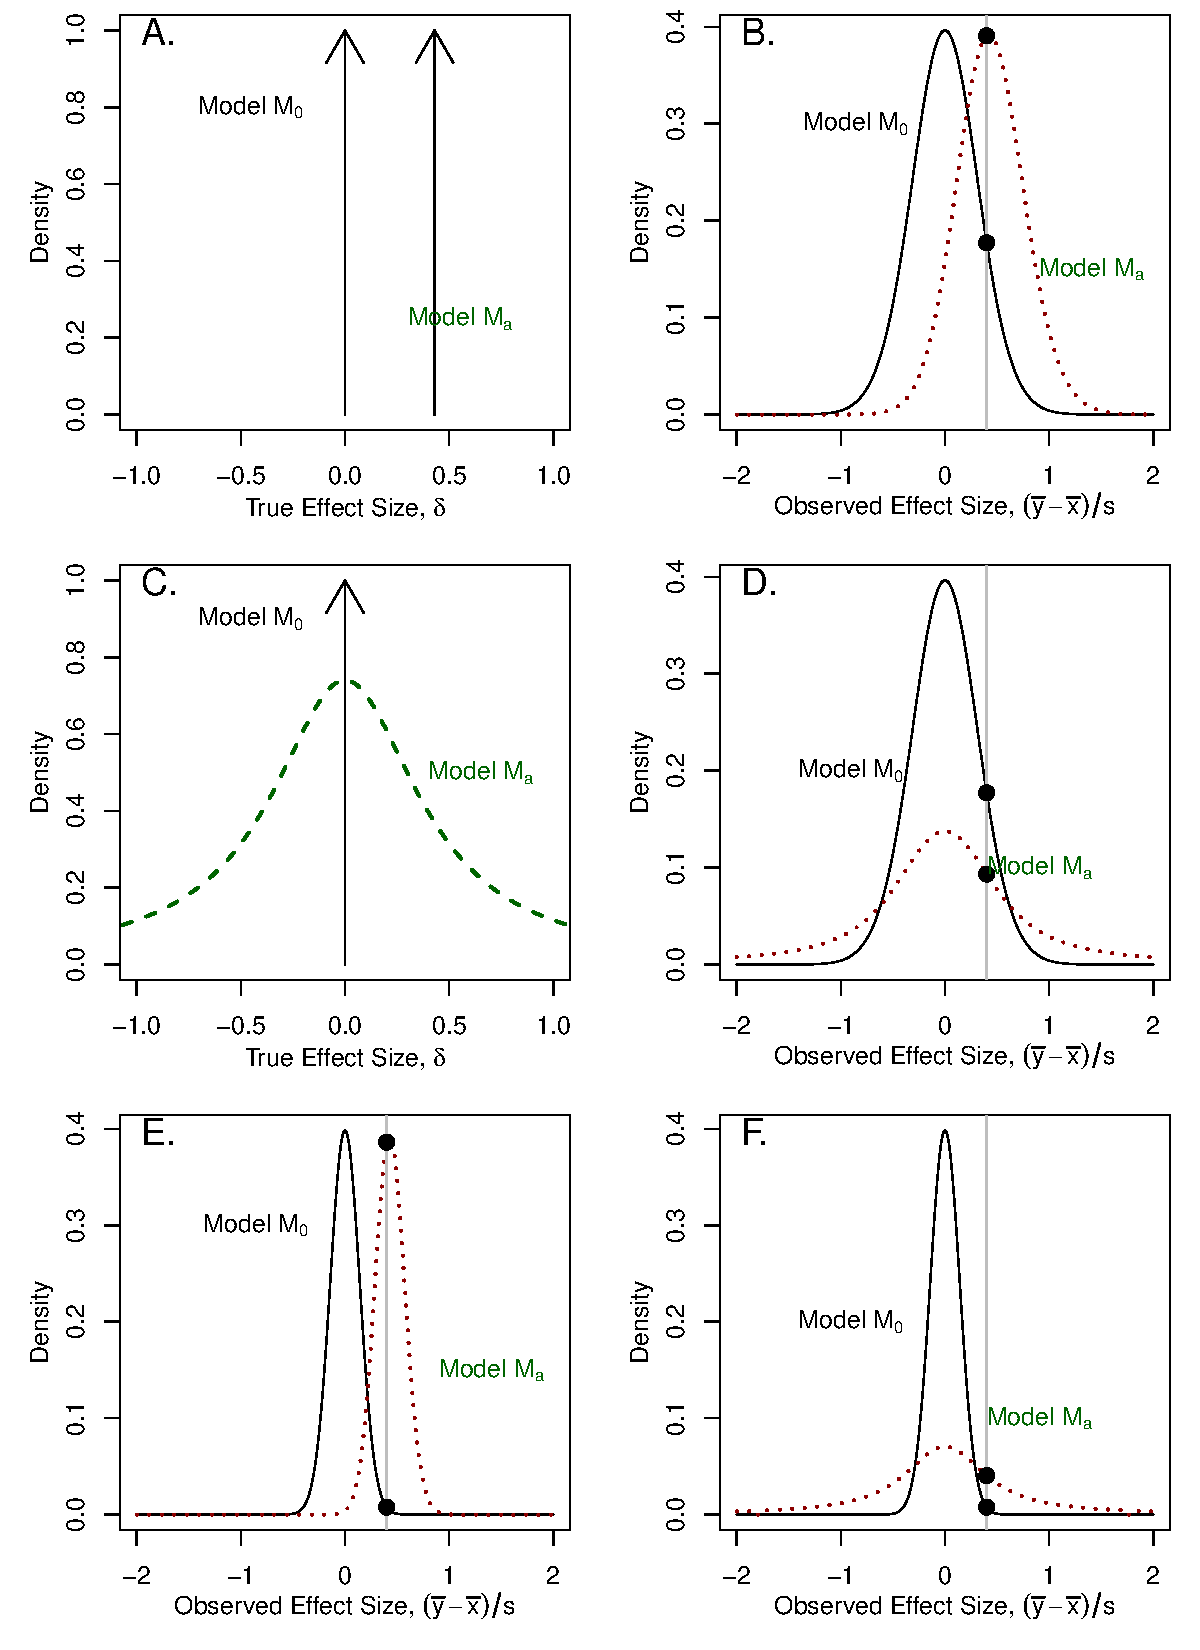
\includegraphics[width=\textwidth, keepaspectratio]{BFfigure.pdf}
\caption{Bayesian model comparison. Panel A shows two point hypotheses $H_0: \delta = 0$ and $H_1: \delta=.43$. Panel B shows the probability of an observed effect size given these hypotheses and a sample of 40 observations between two cells. For an observed effect size $\hat{\delta} = 0.1$, indicated by the vertical grey line, the Bayes factor $B_{01}$ is the ratio of the probabilites, $0.38 / 0.23 = 1.6$. Panel C shows a null hypothesis and a distributed alternative hypothesis $H_1: \delta \sim \mbox{Cauchy(.4)}$. Panel D shows the probabilities of the observed effect size given these hypotheses and a sample of 40 observations between two cells. Panels E and F recreate Panels C and D, respectively, with a larger sample of two hundred observations.}
\label{BFfig}
\end{figure}

\begin{figure}
\includegraphics[width=\textwidth, keepaspectratio]{BFfigure2.pdf}
\caption{Bayes factors by effect size and sample size. Panel A shows the Bayes factor for the point-alternative hypothesis $H_1: \delta = .43$. Panel B shows the Bayes factor for the distributed alternative hypothesis $H_1: \delta \sim \mbox{Cauchy(.5)}$. Solid lines indicate Bayes factors for a small sample of forty observations while dashed lines represent Bayes factors for a larger sample of four hundred observations.}
\label{BFNfig}
\end{figure}


\begin{singlespace}
\begin{table}
\caption{Bayesian results of pilot tests of stimulus equivalence}
\begin{center}
\begin{tabular}{lcccc} 
&$t$&$p$&$\hat{\delta}$&$B_{01}$ \\ \hline
\multicolumn{5}{c}{Arriaga et al., 2008} \\
Difficulty&2.63&.017&1.25&1-to-3.6 \\
Competence&2.27&.035&1.06&1-to-2.1 \\
Discomfort&1.67&.110&0.80&1.1-to-1 \\ 
Realism&1.56&.135&0.75&1.3-to-1 \\
Frustration&1.32&.201&0.63&1.6-to-1 \\
Pleasure&1.29&.214&0.61&1.7-to-1 \\
Action&1.24&.229&0.58&1.8-to-1 \\
Disorientation&1.14&.267&0.54&1.9-to-1 \\ 
Excitement&0.89&.385&0.43&2.4-to-1 \\
Identification&0.86&.398&0.41&2.4-to-1 \\
Satisfaction&0.83&.419&0.39&2.5-to-1 \\ 
Boredom&0.79&.437&0.37&2.5-to-1 \\ 
Presence&0.53&.601&0.24&2.9-to-1 \\
Involvement&0.48&.634&0.22&2.9-to-1 \\
\multicolumn{5}{c}{Anderson et al., 2004}\\
Action&2.35&.028&1.01&1-to-2.4 \\
Difficulty&1.00&.327&0.43&1.6-to-1 \\
Frustration&-0.79&.436&-0.34&1.8-to-1 \\
Enjoyment&-0.40&.693&-0.16&2.0-to-1 \\
Violence&5.48&$<.001$&2.34&1-to-720 \\ \hline
\end{tabular}
\end{center}

\vspace{4mm}
Pilot test results from \citet{Arriaga:etal:2008} and \citet{Anderson:etal:2004}. Pilot data is largely agnostic between the null and alternative, and in fact sometimes indicates equally strong evidence of certain confounds. {\em Note:} $B_{01}$ ranges from 1-to-$\infty$ (perfect evidence for alternative) to $\infty$-to-1 (perfect evidence for null). $H_0: \delta = 0$; $H_1: \delta \sim Cauchy(.5)$. All Bayes factors rounded to two significant digits.
\label{ArriagaAndersonPilot}
\end{table}
\end{singlespace}


\begin{table}
\caption{Results of pilot test from Valadez and Ferguson (2012).} 

\begin{tabular}{l@{\hspace{1cm}} cc@{\hspace{1cm}} cc@{\hspace{1cm}} cc}
& \multicolumn{2}{c}{Difficulty} & \multicolumn{2}{c}{Pace} & \multicolumn{2}{c}{Competitiveness} \\
\cline{2-3} \cline{4-5} \cline{6-7} 
& $t$ & $BF_{01}$ & $t$ & $B_{01}$ & $t$ & $B_{01}$ \\ \hline
Active vs. Control1 & 1.82 & 1-to-1.3 & 1.31 & 1.3-to-1 & 3.00 & 1-to-6.5 \\
Active vs. Control2 & -1.47 & 1.1-to-1 & -2.00 & 1-to-1.6 & 0.05 & 2.1-to-1 \\
Control1 vs. Control2 & -3.45 & 1-to-14 & -3.43 & 1-to-14 & -3.00 & 1-to-6.5 \\
\end{tabular}

Pilot testing suggests that the conditions are different, not equivalent, on ratings. 
{\em Note:} $BF_{01}$ ranges from 1-to-$\infty$ (perfect evidence for alternative) to $\infty$-to-1 (perfect evidence for null). $H_0: \delta = 0$; $H_1: \delta \sim \mbox{Cauchy(.5)}$. All Bayes factors rounded to two significant digits.

\label{ValadezFergusonPilot}
\end{table}

\begin{table}
\caption{Bayesian re-analysis of claimed null results.}
\begin{tabular}{lccccc}
&$\hat{\delta}$   &95\% CI&$n$  &$B_{01}$ & $B_{02}$ \\ \hline
\multicolumn{6}{c}{Aggressive Affect}\\
Anderson et al., 2010, Meta-analysis&0.61&[0.52, 0.72]&2513&-&- \\
\hspace{.2in} Valadez \& Ferguson, 2012&0.45&[0.04, 0.85]&100&1-to-2.3&1-to-8.5 \\
\hspace{.2in} Przybylski et al., 2014, S1&0.00&[-0.39, 0.41]&99&3.0-to-1&62-to-1 \\
\hspace{.2in} Przybylski et al., 2014, S2&0.16&[-.22, .56]&101&2.3-to-1&7.1-to-1 \\
\hspace{.2in} Przybylski et al., 2014, S5&.06&[-0.32, 0.45]&109&3.0-to-1&38-to-1 \\
\hspace{.2in} Ivory \& Kalyanaraman, 2007&0.26&[-0.10, 0.63]&120&1.44-to-1&1.8-to-1 \\
\multicolumn{6}{c}{Aggressive Behavior}\\
Anderson et al., 2010, Meta-analysis&0.43&[0.35, 0.52]&1454&-&- \\
\hspace{.2in} Elson et al., 2014, Noise Intensity&0.41&[-0.04, 0.85]&84&1-to-1.3&1-to-5.1 \\
\hspace{.2in} Elson et al., 2014, Noise Duration&0.22&[-0.22, 0.65]&84&1.9-to-1&1-to-1.1 \\
\hspace{.2in} Ferguson et al. 2008, Study 1 &0.04&[-0.54, 0.65]&50&2.3-to-1&2.4-to-1 \\
\hspace{.2in} Ferguson \& Rueda, 2010 &0.02&[-0.43, 0.47]&77&2.7-to-1&4.4-to-1 \\
\hspace{.2in} Adachi \& Willoughby, 2011, S1&0.00&[-0.63, 0.63]&42&2.2-to-1&2.4-to-1 \\
\hspace{.2in} Adachi \& Willoughby, 2011, S2&0.06&[-0.45, 0.58]&60&2.4-to-1&2.5-to-1 \\
\hspace{.2in} Tear \& Nielsen, 2014 &0.02&[-0.35, 0.39]&120&3.6-to-1&9.0-to-1 \\
\multicolumn{6}{c}{Aggressive Cognition}\\
Anderson et al., 2010, Meta-analysis&0.45&[0.37, 0.52]&2887&-&- \\
\hspace{.2in} Ivory \& Kalyanaraman, 2007&-0.16&[-0.52, 0.22]&120&2.4-to-1&130-to-1 \\ \hline
\end{tabular}

\vspace{4mm}
Some studies present only modest evidence against the effect, and several indicate evidence for the effect despite nonsignificant p-values. 
{\em Note:} $B_{01}$ = evidence for $H_0: \delta = 0$ compared to $HA_1: \delta \sim$ Cauchy(0.4). $B_{02}$ = evidence for $H_0: \delta = 0$ compared to $H_{A2}: \delta \sim \mbox{Normal}(\mu, \sigma)$, with $\mu$ and $\sigma$ taken from \citet{Anderson:etal:2010}. Bayes factors range from 1-to-$\infty$ (perfect evidence for alternative) to $\infty$-to-1 (perfect evidence for null). All Bayes factors rounded to two significant digits. Valadez and Ferguson (2012) effect size is the 2 (Game: {\em Red Dead Redemption, FIFA}) x 2 (Time: pre-, post-) interaction effect. Ferguson et al. (2008) effect size is of those 50 subjects who were randomly assigned to play a violent or nonviolent game. Ferguson and Rueda (2010) effect size is the complex contrast between those participants who played a violent game vs. those who played a nonviolent game. Tear and Nielsen (2014) effect size is the complex contrast between those participants who played a violent game vs. those who played a nonviolent game.
\label{mainStudyResults}
\end{table}

\begin{table}
\caption{Flexible analysis influences Bayes factors, too.}
\begin{center}
\begin{tabular}{lccc}
Quantification&$\hat{\delta}$&$B_{01}$&$B_{02}$ \\ \hline
Mean volume&0.41&1-to-1.2&1-to-4.8 \\
Mean volume after wins&0.26&1.6-to-1&1-to-1.6 \\
Mean volume after losses &0.45&1-to-1.7&1-to-7.2 \\
Mean duration &0.22&2.0-to-1&1-to-1.0 \\
Mean duration after wins&0.10&2.6-to-1&2.7-to-1 \\
Mean duration after losses &0.28&1.5-to-1&1-to-1.9 \\
Mean volume x duration &0.37&1.0-to-1&1-to-3.7 \\
Mean volume x sqrt(duration)&0.37&1.0-to-1&1-to-3.6 \\
Mean volume x ln(duration) &0.32&1.3-to-1&1-to-2.5 \\ 
Count high volume settings &0.87&1-to-140&1-to-279 \\
Count high duration settings &0.10&2.6-to-1&2.8-to-1 \\
First-trial volume &0.06&2.7-to-1&3.5-to-1 \\ 
First-trial duration&0.02&2.8-to-1&4.9-to-1 \\
Count low volume settings&-0.72&1-to-19&1400-to-1 \\
\end{tabular}
\end{center}

\vspace{4mm}
Bayes factors for each effect size as calculated by \citet[study 2, table 2]{Elson:etal:2014}. As pointed out by these authors, the various approaches to quantifying the results of the Competitive Reaction Time Task measure of aggression can lead to very different research conclusions. Bayes factors are not immune to problems of flexible analysis and reporting. {\em Note:} $B_{01}$ = evidence for $H_0: \delta = 0$ compared to $HA_1: \delta \sim$ Cauchy(0.4). $B_{02}$ = evidence for $H_0: \delta = 0$ compared to $H_{A2}: \delta \sim \mbox{Normal}(\mu, \sigma)$, with $\mu$ and $\sigma$ taken from \citet{Anderson:etal:2010}. Bayes factors range from 1-to-$\infty$ (perfect evidence for alternative) to $\infty$-to-1 (perfect evidence for null). All Bayes factors rounded to two significant digits.
\label{ElsonCRTTHacking}
\end{table}

\newpage
\bibliographystyle{apacite}
\bibliography{database}
\end{document}

% % % % % % % % % % % %
% Supplementary tables %
% % % % % % % % % % % % %

% need to change these to delta as well

\begin{singlespace}
\begin{table}
\caption{Results of pilot tests for equivalence with null interval}
\begin{center}
\begin{tabular}{lcccc} 
&$t$&$p$&$\hat{\delta}$&$B_{01}$ \\ \hline
\multicolumn{5}{c}{Arriaga et al., 2008} \\
Difficulty&2.63&.017&1.25&1-to-4.0 \\
Competence&2.27&.035&1.06&1-to-2.2 \\
Discomfort&1.67&.110&0.80&1.1-to-1 \\ 
Realism&1.56&.135&0.75&1.3-to-1 \\
Frustration&1.32&.201&0.63&1.8-to-1 \\
Pleasure&1.29&.214&0.61&1.9-to-1 \\
Action&1.24&.229&0.58&2.0-to-1 \\
Disorientation&1.14&.267&0.54&2.2-to-1 \\ 
Excitement&0.89&.385&0.43&2.9-to-1 \\
Identification&0.86&.398&0.41&3.0-to-1 \\
Satisfaction&0.83&.419&0.39&3.1-to-1 \\ 
Boredom&0.79&.437&0.37&3.2-to-1 \\ 
Presence&0.53&.601&0.24&3.9-to-1 \\
Involvement&0.48&.634&0.22&4.0-to-1 \\
\multicolumn{5}{c}{Anderson et al., 2004}\\
Action&2.35&.028&1.01&1-to-2.6 \\
Difficulty&1.00&.327&0.43&1.7-to-1 \\
Frustration&-0.79&.436&-0.34&2.0-to-1 \\
Enjoyment&-0.40&.693&-0.16&2.4-to-1 \\
Violence&5.48&$<.001$&2.34&1-to-818 \\ \hline
\end{tabular}
\end{center}

\vspace{4mm}
Pilot test results from \citet{Arriaga:etal:2008} and \citet{Anderson:etal:2004}. Pilot data is largely agnostic between the null and alternative, and in fact sometimes indicates equally strong evidence of certain confounds. {\em Note:} $B_{01}$ ranges from 1-to-$\infty$ (perfect evidence for alternative) to $\infty$-to-1 (perfect evidence for null). Contrary to the authors' original conclusions, the pilot test has some evidence the games differ in feelings of competence, and fairly substantial evidence that they differ in difficulty. $H_0: \delta \sim \mbox{Uniform(-0.1, 0.1)}$; $H_1: \delta \sim Cauchy(.5)$. All Bayes factors rounded to two significant digits.
\label{ArriagaAndersonPilot_NullInterval}
\end{table}
\end{singlespace}

% Is this table legible?
\begin{table}
\caption{Results of Pilot Tests from Valadez and Ferguson (2012) with null interval.} 

\begin{tabular}{l@{\hspace{1cm}} cc@{\hspace{1cm}} cc@{\hspace{1cm}} cc}
& \multicolumn{2}{c}{Difficulty} & \multicolumn{2}{c}{Pace} & \multicolumn{2}{c}{Competitiveness} \\
\cline{2-3} \cline{4-5} \cline{6-7} 
& $t$ & $BF_{01}$ & $t$ & $B_{01}$ & $t$ & $B_{01}$ \\ \hline
Active vs. Control1 & 1.82 & 1-to-1.3 & 1.31 & 1.3-to-1 & 3.00 & 1-to-7.2 \\
Active vs. Control2 & -1.47 & 1.1-to-1 & -2.00 & 1-to-1.6 & 0.05 & 2.5-to-1 \\
Control1 vs. Control2 & -3.45 & 1-to-16 & -3.43 & 1-to-15 & -3.00 & 1-to-7.2 \\
\end{tabular}

Pilot testing suggests that the conditions are different, not equivalent, on ratings. 
{\em Note:} $BF_{01}$ ranges from 1-to-$\infty$ (perfect evidence for alternative) to $\infty$-to-1 (perfect evidence for null). $H_0: \delta \sim \mbox{Uniform(-0.1, 0.1)}$; $H_1: \delta \sim \mbox{Cauchy(.5)}$. All Bayes factors rounded to two significant digits.

\label{ValadezFergusonPilot_NullInterval}
\end{table}